\cotefile{150}

\scanpage{25}
\diagram{
\begin{tikzcd}[column sep=small,row sep=small]
\dot T\cap E\simeq\dot T_0\times I
\arrow[dr,phantom,"\subset" sloped] & \\
\text{\deleted{\unsure{et si|et où}}} & T\cap E\simeq T_0\times I \\
Y\cap E\unsure{\}}\simeq Y_0\cap E
\arrow[ur,phantom,"\subset" sloped] & \\
\unsure{\vert|1} &
\end{tikzcd}
\(\qquad\text{où}\qquad
\begin{aligned}
\dot T_0&=\dot T\cap X_0\\
T_0&=T\cap X_0\\
Y_0&=Y\cap X_0
\end{aligned}\)
}

et si, symétriquement,
\deleted{$\unsure{T\cap E},T\cap\dot E,X_0\quad T\cap E$}

b) $E\cap T\ (=T\cap E)$, $\dot E\cap T\deleted{\simeq T_0\times\{1}$,
$X_0\cap T\ (=T\cap X_0=T_0)$ sont des
sous-espaces côniques de $T$, donc en particulier
stables par $T$-homothéties. \deleted{Le fait que} Noter que
les trois espaces précédents s'identifient, grâce à a),
à $T_0\times I$, $T_0\times\{1\}$, $T_0\times\{0\}$. On suppose enfin

c) Les homothéties \deleted{par} $\lambda_E$ et $\lambda_T$ \inserted{commutent}
dans $T\cap E$, ce qui implique que l'application
\deleted{$\lambda_T$} induite par $\lambda_T$ ($\lambda\in[0,1]$) sur
$T_0\times\{0\}$ et $T_0\times\{1\}$
s'identifie à une $=$ \deleted{homothétie} opération de
$T_0\unsure{-|\to}T_0$, \deleted{et que} soit $\lambda_{T_0}$, et que l'opération
$\lambda_T$ sur $T\cap E\simeq T_0\times I$ s'identifie \unsure{à|:}
\deleted{$\unsure{\lambda_{T_0}}$} $\lambda_{T_0}\times\operatorname{id}_I$.

Donc les conditions a) b) c) équivalent à celle-ci :

\uline{Condition de compatibilité} $\exists$ homéomorphisme
\[
T\cap E\simeq T_0\times I
\qquad\text{(compatible avec }E\simeq X_0\times I
\]
\deleted{compatible \unsure{aux structures|avec structure}}
induisant
\[
\dot T\cap E\simeq\dot T_0\times I,\qquad Y\cap E\simeq Y_0\times I
\]
\unsure{tels|tel} que la structure cônique de $T$ sur $Y$
\unsure{induite|s'identifie} sur $T_E$ sur $Y_E$
\deleted{avec \unsure{de} la} \inserted{une}
\uline{structure cônique produit} \inserted{par $I$,}
d'une structure cônique de
$T_0$ sur $Y_0\subset T_0$, \deleted{par $I$}
\margin{24}

\scanpage{26}
\mspage{8}
\uline{NB} Cette condition implique que pour $\lambda_0,\lambda'_0\in\unsure{]0,1]|[0,1]}$,
$\underset{E}{\lambda_0}E$ et $\underset{T}{\lambda'_0}T$ sont compatibles.

Si $T$ est aussi cylindrique, la condition
envisagée de compatibilité de deux structures
cylindriques est symétrique.

\inserted{\uline{Prop}}
Si $(X,Y,\mathcal T)$ est décrit par $(\widetilde X,\dot X,\mathcal E_{\dot X},Y,\dot X\to Y)$,
lors \inserted{les} $(X_0,\mathcal E)$ \inserted{germes de} structures cylindriques compatibles
avec le germe de structure cône $\mathcal T$ correspondent
aux \deleted{couples}\inserted{systèmes}
$(\widetilde X_0,\widetilde{\mathcal E}_{\widetilde X_0}\deleted{\unsure{\}|)}},Y_0,\mathcal E_{Y_0})$
où $\widetilde X_0$ est une partie bordante de \deleted{$\unsure{X_0|\mathcal E_{X_0}}$} $\widetilde X$, munie
d'un germe de voisinage cylindrique $\widetilde{\mathcal E}_{\widetilde X_0}$,
où $Y_0$ est une partie bordante de $Y$, munie d'
un germe de \deleted{\unsure{vois.|voisin}} voisinage cylindrique
$\mathcal E_{Y_0}$, \unsure{ces|les} données satisfaisant aux conditions
suivantes :

a) $\widetilde{\mathcal E}_{\widetilde X_0}$ et $\mathcal E_{\dot X}$ sont des
\inserted{germes de} structures cylindriques
\uline{compatibles} --- donc $\underset{\inserted{\substack{\Vert\\\widetilde X_0\cap\dot X}}}{\dot X_0}\subset\dot X$
hérite d'un
germe de structure cylindrique \inserted{dans $\dot X$} (induit par
$\widetilde{\mathcal E}_{\widetilde X_0}$)

b) Le morphisme
\deleted{$(\dot X,\unsure{\mathcal E})\longrightarrow(Y,$}
\inserted{$\dot X\overset{p}{\longrightarrow} Y$}
est compatible
avec $(\dot X_0,\mathcal E_{\dot X_0})$ et $(Y_0,\mathcal E_{Y_0})$, dans le sens
évident \inserted{que $\dot X_0=\unsure{p|\beta}^{-1}(Y_0)$, \uline{et}}
qu'il existe des voisinages cylindriques
représentatifs des deux germes envisagés
\[
\deleted{\unsure{\dot X_0|X_0}}\quad
E_{\dot X}\simeq\dot X_0\times I,\qquad E_Y\simeq Y_0\times I,
\]
tels que
\margin{25}

\scanpage{27}
$p|_{\dot X_0\times I}$ induise $\dot X_0\times I_{\unsure{2|\ell}}\longrightarrow Y_0\times I$,
s'identifiant à $p_0\times\operatorname{id}_I$, où $p_0:X_0\longrightarrow Y_0$.

\deleted{Compatibilité}\inserted{Transversalité} d'une famille \deleted{finie}
$(B_i,E_{B_i})$ de voisinages cylindriques \unsure{des|de} parties $B_i$ de $X$.
La condition s'exprime en disant que pour
tout $J\subset I$, $I$ fini, la structure de
\[
\bigcap_{i\in J}E_{B_i}\overset{\mathrm{def}}=E_J,
\quad\text{\unsure{autour|au dessus} de}\quad
B_J\overset{\mathrm{def}}=\bigcap_{i\in J}B_i,
\]
est celle de $B_J\times I^J$, l'homothétie
$\lambda_{E_j}$ de $E_j$ \inserted{(pour $j\in J$)} induisant
\[
(b,(t_\alpha)_{\alpha\in J})\longmapsto(b,\unsure{(t'_\alpha)|(t'_\alpha]}),
\qquad
t'_\alpha=t_\alpha\ \text{si }\alpha\ne j,\quad
\text{et }\unsure{t'_\alpha|t_\alpha}=\lambda t_\alpha\ \text{si }\alpha=j.
\]
\margin{cet homéom. $E_J\simeq B_J\times I^J$ est
canonique, si
$\dot B_J=\bigcap_{j\in J}\dot E_j
\underset{\substack{\text{\unsure{multiplié}}\\
\text{\deleted{\unsure{par}\ \illegible{1}}}\\
\text{l'élément \unsure{unité|nul} de}\\I^J}}{\xrightarrow{\sim}}B_J$
\ldots}

Cela peut aussi s'expliciter en exigeant
que $E_J$ soit cylindrique dans chaque $E_{B_j}$ etc\ldots
Cette relation de transversalité passe aux germes.

On dit que la famille précédente \uline{et}
un voisinage conique $T$ de $Y\subset X$ sont
\inserted{transversaux} \deleted{\unsure{compatibles|compatible}}
si \deleted{la structure des $T\cap E_i$}
\inserted{\uuline{de plus} $\forall\deleted{\unsure{j}}J$ comme dessus,}
\margin{\unsure{induit par} \unsure{\(\mathinner{\cdotp-\cdotp}\)}
$E_J\simeq B_J\times I^J$ et}
\[
\begin{array}{l@{\quad}lcl@{\quad}l}
& E_J\cap T & \simeq & T_J\times I^J
& (\text{où }T_J=T\cap B_J)\\
&\cup&&\cup&\\
\text{induisant}&\dot E_J\cap\dot T&\simeq&\dot T_J\times I^J
&(\text{où }\dot T_J=\dot T\cap B_J)\\
&E_J\cap Y&\simeq&Y_J\times I^J
&(\text{où }Y_J=Y\sim B_J)
\end{array}
\]
\margin{26}

\scanpage{28}
\mspage{9}
avec $E_J\cap T$ cônique dans $T$, et la structure côniq
\deleted{induit} étant la structure produit par $I^J$ d'
une structure cônique sur $(T_J,Y_J)$, ayant
$\dot T_J$ comme partie-bord du cône sur $Y_J$\(\mathinner{\cdotp\cdotp-}\).

\deleted{\unsure{6}}

\textcircled{6.} Relations aux stratifications de type $I$
($I$ ens ordonné fini)
Une telle stratification (d'un espace $X$) est
la donnée d'une famille croissante de
sous-espaces fermés $X_i$. On dit que
la stratification est \uline{précylindrique} si

\deleted{$\forall i$}
a) $\forall j'\leftrightarrow j$, $j$ successeur de $j'$,
$X_{j'}\hookrightarrow X_j$ est
\deleted{\unsure{une part.}} \inserted{bordant}

\inserted{b) \deleted{\unsure{Pour}}\inserted{Pour} $j$ fixé,
$j'$ variable parmi les prédécesseurs, les
$X_{j'}$ sont des parties \unsure{bordantes} transversaux de $X_j$}

\margin{i.e. munis des voisinages cylindriques transversaux}

\deleted{b)}\inserted{c)}
$\forall i\leftrightarrow j$, la structure de l'ens \inserted{$I_{i,j}$}
des $k$ tels que $i\le k\le j$ est celle de l'ens
\inserted{parties d'un ens} \deleted{simplexe} --- ce qui signifie que
si $S\inserted{(=S_{ij})}$ est l'ens. des prédécesseurs de $j$ dans
$I_{i,j}$ \inserted{i.e. des éléments minimaux de $I_{i,j}\setminus\{j\}$}
et si pour \unsure{$\forall$} $k\in I_{i,j}$, on désigne
\deleted{\unsure{alors}} par $s_k$ \deleted{l'ens des}\inserted{la} \unsure{parties|partie} $s_k\subset S$ formée
de $j\in S_{\unsure{k}}$ tels que
$j\ge s_k$ (donc $s_k=s_{kj}$)
l'application $k\longrightarrow s_k$ (qui est décroissante)
est un antiisomorphisme de $I_{ij}$ avec $\mathcal P(S)$
ordonné par inclusion. \deleted{$\unsure{I}$}

\margin{\uline{NB} Compte tenu de c), il suffit d'exiger dans
b) pour $j$ maximal \unsure{dans $I$.}}

\margin{\deleted{\unsure{dans un même cône}}
\inserted{\deleted{\unsure{des parties}}}}

\margin{On veut de plus \deleted{\unsure{que}}
que les Inf dans $I_{i,j}$ correspond\unsure{ent} à
l'intersection des $X_k$\(\mathinner{\cdotp-\, -}\) cf. (0) ci-dessous.}

Combinant b) et c), on voit que le
\margin{27}

\scanpage{29}
structure locale de $X_j$ le long d'un $X_i$
(avec la stratification induite de type $I_{ij}$)
est ``cubique''
(coin de cube de
dimension $n=\operatorname{card}S$)

\figure{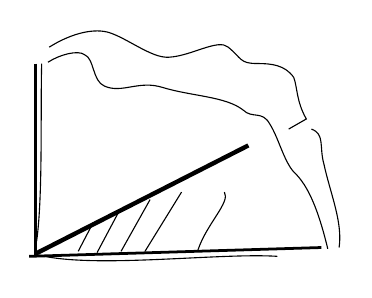
\begin{tikzpicture}[x=0.016cm,y=-0.016cm]
\draw[line width=1pt] (21,35)--(21,187);
\draw (26,35) .. controls (25,75) and (27,140) .. (22,176);
\draw[line width=1pt] (16,188)--(248,181);
\draw (24,187) .. controls (68,198) and (167,185) .. (213,188);
\draw (31,34) .. controls (40,28) and (55,24) .. (60,28)
.. controls (68,31) and (66,49) .. (76,53)
.. controls (90,59) and (103,48) .. (122,54)
.. controls (145,61) and (172,61) .. (186,72)
.. controls (193,79) and (201,72) .. (207,83)
.. controls (214,94) and (218,112) .. (226,121)
.. controls (238,132) and (246,153) .. (253,182);
\draw (32,22) .. controls (48,12) and (65,7) .. (78,10)
.. controls (93,14) and (113,31) .. (127,30)
.. controls (145,29) and (166,15) .. (174,22)
.. controls (185,31) and (183,35) .. (197,35)
.. controls (208,35) and (219,36) .. (226,46)
.. controls (229,54) and (228,65) .. (236,79)
--(222,87);
\draw (240,87) .. controls (251,91) and (246,101) .. (250,115)
.. controls (255,138) and (265,161) .. (262,181);
\draw[line width=1.6pt] (21,186)--(190,100);
\draw (55,184)--(67,161);
\draw (70,185)--(87,153);
\draw (89,184)--(112,143);
\draw (108,184)--(137,137);
\draw (150,183) .. controls (157,162) and (176,145) .. (171,137);
\end{tikzpicture}}

La \deleted{condition} \inserted{c)} \unsure{impliquent|implique} que si $j'$ est
un prédécesseur de $j$, et si $k\in I$ est $\le j$
mais non $\le j'$, et s'il existe
un $i$ majoré par $k$ et $j'$, \uline{alors}
$k'=\operatorname{Inf}(k,j')$ existe, et $k'$ est
un prédécesseur de $k$.

\diagram{\begin{tikzcd}[column sep=small,row sep=small]
& j' \arrow[r,leftrightarrow,"\mathrm{préd}"'] \arrow[d,phantom,"{\rotatebox{90}{$\leq$}}" description] & j \arrow[d,phantom,"{\rotatebox{90}{$\leq$}}" description] \\
& k' \arrow[r,leftrightarrow] & k \\
i \arrow[uur,hook] \arrow[urr,hook] & &
\end{tikzcd}}

(Il suffit de voir que dans
un ens. ordonné de la forme $\mathcal P(\unsure{\sigma|F})$,
les inf exist (c'est l'intersection) et si
$j'\subset j=j'\amalg\{\alpha\}$, et $k\in j$ mais non $k\subset j'$,
alors \deleted{$\unsure{k\ne k'}$} $k=k'\amalg\{\alpha\}$ avec $k'=k\cap j'$, ..)
\margin{$\sigma$ ens fini}

Ceci posé, considérons le diagramme
\diagram{\begin{tikzcd}
X_{j'} \arrow[r,hook] & X_j \\
X_{k'} \arrow[u] \arrow[r,hook] & X_k \arrow[u]
\end{tikzcd}}
où les flèches verticales, par l'hyp. $\unsure{1^\circ)|16)}$,
sont des plongements bordants. Ceci posé, on
voit \inserted{(par b,c)} que \deleted{$(X_k\longrightarrow X_{\unsure{j}}$.}
$(X_k,X_{k'})\mathbin{-}(X_j,X_{j'})$
\margin{28}

\scanpage{30}
7. \uline{Stratifications} et \uline{voisinages côniques} : le pas
de récurrence.

$(X_i)_{i\in I}$, famille croissante de parties de $X$,
satisfaisant
\[
(14)\qquad\text{a) }\forall i,j\in I,\ \text{on a}\qquad
X_i\cap X_j=\bigcup_{\alpha\le i,j}X_\alpha.
\]
\inserted{b) $X=\bigcup_{i\in I}X_i$}

\margin{Cette condition se généralise :
aux intersections quelconques
$\displaystyle\bigcap_{i\in J}X_i=
\bigcup_{\unsure{\{}\,\substack{k\in I\\k\text{ minorant }J}}X_k$}

Transversalité : un syst. de parties-bord \inserted{$B_\alpha$} de
$X$, muni de germes de cylindres associés
(mutuellement transversaux entre eux) : si on
représente les germes par des cylindres convenable\unsure{s}
$E_{B_\alpha}$, imposant\inserted{exprimant} que les $X_i$ soient transversaux
aux \unsure{l'}$E_{B_\alpha}$ --- cela implique que l'on a
\[
E_J\cap X_i\simeq (X_{iJ}\times I^J
\qquad
\text{(induit par }E_J\simeq B_J\times I^J,
\]
avec $X_{iJ}=X_i\cap B_J$).
\deleted{Bien sûr les}
\margin{pour $J$ \deleted{\unsure{ensemble}} ensemble d'indices $\alpha$}

\deleted{\unsure{Soit}}
Soit $I_0\subset I$ une partie de $I_0$ formée
d'éléments minimaux, \deleted{et \unsure{soit}} et soit
\[
X_{I_0}=\bigcup_{i\in I_0}X_i=\coprod_{i\in I_0}X_i
\]
\deleted{\unsure{Alors}}
La donnée d'un germe \deleted{de structure}
d'un voisinage cônique \inserted{strict} de $X_{I_0}$ équivaut \unsure{à|:}
celle d'un syst de voisinages côniques
$T_i$ ($i\in I_0$) mutuellement disjoints des $X_i$ ---
celle d'un germe de voisinage cônique de $X$,
à celle d'une famille de germes de vois.
côniques des $\unsure{X_i|X}$ dans $X$.
\margin{29}

\scanpage{31}
\mspage{10}
est ``transversal'' i.e. \deleted{\unsure{X|si}} $\exists$ voisinages cylindriques
de $X_{j'}$ \inserted{\unsure{de|dans} $\unsure{X_j,|X_{j\prime}}$} et un de $X_{k'}$ dans $X_k$, tel que l'application
$X_k\unsure{-|\to}X_j$ induit un \deleted{hom}\inserted{morphisme} sur les
cylindres (compatible avec les structures
cylindriques) et de plus
$E_{k',k}=p_{jk}^{-1}(\overline E_{j',j})$.

Système de voisinages cylindriques \deleted{\unsure{associé}}
\inserted{(des $X_{j'}$ dans les $X_j$)}
compatible avec une stratification : tel que
dans b, les \deleted{$X$}$E_{j',j}$ ($j$ fixé, $j'$ prédécesseur)
soient compatibles. Notion correspondante
pour les germes de voisinage cylindrique.

Stratification cylindrique : stratification munie
d'une telle ``structure cylindrique'', en
termes de germes de voisinages cylindriques.

\deleted{\uline{NB} Une}
\uline{NB} Une stratification précylindrique \inserted{resp. cylindrique}
est sûrement
``\unsure{équisingulier|équisingulière}'' au sens le plus fort qu'on
puisse introduire $\to$ (\unsure{C|cf.}) suite.

Mais j'ai oublié une condition, que j'exigerai
pour tte stratification :
\[
(0)\qquad \forall i,j\in I,\quad\text{on a}\quad
X_i\cap X_j=\bigcup_{k\le i,j}X_k
\]
\margin{\uline{NB} si $i,j$ ont pour borne inf $h$,
cela implique $X_i\cap X_j=X_h$. \unsure{même pour} \illegible{3} \unsure{c)} $\unsure{X_i\cap X_j}$.}

Corollaire : Si $X_i\cap X_j\ne\phi$, alors $i,j$ ont un
minorant $h$ (tel que \deleted{\unsure{le}} $X_k\unsure{\}}\ne\phi$\(\mathinner{\cdotp-\, -}\))
\margin{30}

\scanpage{32}
\mspage{11}
Prenons $T_{I_0}=\coprod_{\beta\in I_0}T_\beta$ voisinage
\deleted{tubulaire}\inserted{cônique} strict
de $X_{I_0}$, supposons le str\textsuperscript{t} transversal aux
$(B_i,\mathcal E_i)$, et \deleted{aux} que les $X_i$
($i\in I^*\overset{\mathrm{def}}=I\setminus I_0$)
soient str. admissibles pour $T_{I_0}$.

Notons que en vertu de (14), si $\beta\in I_0$ donc
minimal dans $I$, donc pour $i\in I$ on a
\[
(14)\qquad
X_i\cap X_\beta=
\begin{cases}
\phi & \text{si }\deleted{\beta}i\not\ge\beta\\
X_\beta & \text{sinon \unsure{i.e.} }i\ge\beta\quad(\text{ceci est trivial})
\end{cases}
\]
Soit $I_\beta$\inserted{$\subset I^*$} l'ens des $i\in I$ tels que $i>\beta$\unsure{.}
On a donc
\[
(15)\qquad i\in I^*\setminus I_\beta\quad\Longrightarrow\quad
X_i\cap T_\beta=\phi
\]
(car $X_i\cap X_\beta=\phi$ et $X_i$ admissible pour $T_\beta$),
\[
(16)\qquad i\in I_\beta\quad\unsure{=|\Longrightarrow}\quad X_i\supset X_\beta
\]
Donc on a
\[
(16')\qquad X_i\cap T_\beta
=I.\underbrace{X_i\cap\dot T_\beta}_{\dot X_i}\cup X_\beta
\]

Ainsi, le système
\[
(17)\qquad
(X,(X_i)_{i\in I},(B_\alpha,\mathcal E_\alpha)_{\alpha\in R}
(\mathcal T_\beta)_{\beta\in I_0})
\]
se reconstitue à l'aide de
\inserted{$\boxed{(X_\beta)_{\beta\in I_0},}$}

\[
\deleted{\begin{gathered}
(18)\quad
\left(
\underset{\substack{\parallel\\X\setminus\mathring T_{I_0}}}{X^*},
\left(\underset{\dot T_\beta}{\dot X_\beta}\right)_{\beta\in I_0},
\left(\underset{\substack{\parallel\\B_\alpha\cap X^*}}{B_\alpha^*},
\underset{\substack{\parallel\\\mathcal E_\alpha\unsure{\mid|\cap}X^*}}{\mathcal E_\alpha^*}\right),
\left(\underbrace{(X_{\beta\alpha},\mathcal E_{\beta\alpha})}
_{=(B_{\unsure{\alpha}}^*,\mathcal E_\alpha^*)|X_\beta}\right)_{\beta\in I_0}
\right)
\\
(\dot X_\beta\longrightarrow X_\beta)_{\beta\in I_0})
\end{gathered}}
\]
\margin{31}

\scanpage{33}
\mspage{12}
\[
(18)\quad\left\{
\begin{gathered}
\underset{\substack{\parallel\\X\setminus\mathring T_{I_0}}}{X^*},
\overbrace{
\left(\underset{\substack{\parallel\\\dot T_\beta}}{\dot X_\beta},
\unsure{\mathcal E_\beta}\right)_{\beta\in I_0},
\underset{(B_\alpha,\mathcal E_\alpha)|X^*}
{\underline{(B_\alpha^*,\mathcal E_\alpha^*)}}{}_{\alpha\in\Lambda}
}^{\substack{\text{syst. de cylindres-bord}\\\text{transversaux}}},
\left(\underset{\substack{\parallel\\X_i\cap X^*}}{X_i^*}\right)_{i\in I^*};
(X_\beta)_{\beta\in I},
\underbrace{(B_{\beta,\alpha},\mathcal E_{\beta,\alpha})}
_{(B_\alpha,\mathcal E_\alpha)|X_\beta}
{}_{\substack{\alpha\in\Lambda\\\beta\in I_0}},\\
(\dot X_\beta\overset{p_\beta}\longrightarrow X_\beta)_{\beta\in I_0}
\end{gathered}\right\},
\]
de la façon suivante :

\margin{les $\dot X_\beta$ disjoints}
\[
(19)\quad\left\{
\begin{aligned}
\widehat X&=X^*\amalg_{\dot X=\coprod\dot X_\beta}
\underbrace{C(p=\coprod p_\beta)}
_{\deleted{\unsure{I}}\coprod_\beta C(p_\beta)},\\
T_\beta&=C(p_\beta)\\
X_\beta&\quad\text{pour }\beta\in I_0\quad\text{clair}.\\
X_i&\quad\text{pour }i\in I^*\text{ est donné par }
\deleted{X_i=I\unsure{.}\underset{\unsure{\parallel\text{def}}}{\underline{\dot X_i}}}\\
\deleted{X_i}\quad\unsure{X_i|\bar X_i}&=X_i^*\deleted{\unsure{\cup}}
\cup\bigcup_{\substack{\beta\in I_0\\\beta\le i\\\deleted{\unsure{i\in I_\beta}}}}
\left(I.\underset{\substack{\parallel\text{déf}\\X_i^*\cap\dot X_\beta}}
{\underline{\dot X_{i\beta}}}
\deleted{\unsure{I.(X_i^*\cap\dot X_\beta)}}\cup X_\beta\right)\\
B_\alpha&=B_\alpha^*\cup\bigcup_{\beta\in I_0}
I\underset{\substack{\parallel\text{déf}\\B_\alpha^*\cap\dot X_\beta}}
{\underline{\dot B_\alpha}}\\
\mathcal E_\alpha&\quad\text{défini par }\mathcal E_\alpha^*
\text{ et les }(B_{\beta,\alpha},\mathcal E_{\beta,\alpha})
\end{aligned}\right.
\]

\uline{Conditions} sur (18)

% The right brace joins a and b; the left brace labelled (20) starts at b.
% Separate curved leader: from the lower-left edge of circled d, down between
% the left brace and the labels, then right beneath the last circled label.
\[
\begin{array}{@{}r@{\;}l@{\;}l@{}}
&\text{\textcircled{a} Les }X_\beta\text{ disjoints}
&\smash{\raisebox{-0.30cm}{$\left.\vphantom{\rule[-0.50cm]{0pt}{1.00cm}}\right\}\Longrightarrow$}}\\[0.45em]
\smash{\raisebox{-1.25cm}{$(20)\left\{\vphantom{\rule[-1.60cm]{0pt}{3.20cm}}\right.$}}
&\text{\textcircled{b} Chaque }\dot X_\beta\text{ transverse \unsure{à|:} }(B_\alpha^*,\mathcal E_\alpha^*)
&\\[1em]
\smash{\raisebox{-2.25cm}{\begin{tikzpicture}[x=1cm,y=1cm]
\draw[->,line width=0.4pt] (0.10,2.50)
.. controls (-0.10,2.30) and (-0.20,1.80) .. (-0.20,1.20)
-- (-0.20,0.25)
.. controls (-0.20,0.00) and (0.20,0.00) .. (0.65,0.00);
\end{tikzpicture}}}
&\text{\textcircled{d}}\quad
(\dot X_\beta,
\underset{\substack{\text{induit sur }\dot X_\beta\\
\text{par }(B_{\unsure{\alpha}},\mathcal E_{\unsure{\alpha}})}}
{\underline{\dot B_{\beta\alpha},\dot{\mathcal E}_{\beta\alpha}}})
\longrightarrow
(X_\beta,B_{\beta,\alpha},\dot{\mathcal E}_{\beta,\alpha})
&\\
&\hspace{5.2cm}\text{est transverse}&\\[1em]
&\inserted{\text{\textcircled{\unsure{c|d}} Les }X_i^*\text{ transverses aux }
\big((\dot X_\beta,\mathcal E_\beta)_{\beta\in I_0},
(B_\alpha^*,\mathcal E_\alpha^*)_{\alpha\in\Lambda}\big)}&
\end{array}
\]
\margin{le syst. des $(\dot X_\beta,\unsure{\mathcal E_\beta}$
$(B_\alpha^*,\mathcal E_\alpha^*)$ est transv\unsure{e}}
\margin{32}

\scanpage{36}
par récurrence sur $\operatorname{card}I$ la notion de
donnée \deleted{de} coniques sur \deleted{cette base}
$(X,(X_i)_{i\in I}(B_\alpha,\mathcal E_\alpha)_{\alpha\in\unsure{\lambda|\Lambda}}$
\deleted{On procède.} Si $I=\phi$, ce sera la structure
vide (il y en a une et une seule). Si
$I\ne\phi$, on prend $I_0$ ens des éléments minimaux
de $I$, et une donnée conique sera par
définition la donnée

\textcircled{a} d'un \deleted{tube}\inserted{vois. con. strict} $T_{I_0}$
de \deleted{\unsure{la somme}} $\deleted{T}X_{I_0}=\bigcup_{\beta\in I_0}X_\beta$,
transversal aux $(B_{\unsure{\bar\alpha}},\mathcal E_\alpha)$ et
\deleted{\unsure{donc} admissible}
coniquement transversal aux $X_i$ ($i\in I$).
--- ce qui permet donc d'introduire les
structures (19), et en particulier

\[
(22)\qquad
X^*,\quad
\underset{\text{stratification de }I^*}{(X_i^*)_{i\in I^*=I\setminus I_0}},
\quad
\underbrace{\big((\deleted{\unsure{\mathcal E}}B_\alpha,\mathcal E_\alpha)_{\alpha\in\Lambda},
(\dot X_\beta,\mathcal E_\beta)_{\beta\in I_0}\big)}
_{\substack{\text{famille \unsure{transverse|transversale}}\\\text{de sous-espaces}\\
\text{\unsure{bordants} ``cylindrisés''}\\
\text{de }X,\ \text{transversaux}\\\text{aux }X_i}}
\]

en plus de
\[
(23)\qquad
(X_\beta)_{\beta\in I_0},
(B_{\beta\alpha},\mathcal E_{\beta\alpha})_{\substack{\beta\in I_0\\\alpha\in\Lambda}}\big)
\]
On doit avoir de plus : $\infty$

\textcircled{b} Une structure conique sur (22) (ce qui
a un sens, par récurrence\ldots)
\margin{35}

\scanpage{37}
\mspage{14}

\deleted{\unsure{NB}}\quad \uline{Remarques}\quad
1) Avec des hypothèses de ``non sauvagerie'' sur la donnée initiale
\[
 (X,(X_i)_{i\in I},(B_\alpha,\mathcal E_\alpha)_{\alpha\in\Lambda}),
\]
il doit être vrai qu'il existe une structure cônique. Si la stratification
\deleted{\unsure{X}} est équisingulière le long de tout
\[
 X_i^\circ\mathrel{\mathop=^{\mathrm{def}}}
 X_i\setminus\bigcup_{\substack{j<i\\j\le i}}X_j,
\]
alors il doit \(=\) y avoir une structure cônique équisingulière
(avec la définition ad-hoc évidente) --- il suffit de savoir construire
un tube équisingulier autour des \(X_{I_0}\) \(\cdots\)

2) A priori, si on a une suite \inserted{str.} croissante
de parties
\[
 \phi\subset I_0\subset I_1-\, -\subset I_{n-1}\subset I_n=I,
\]
avec \deleted{\(I_i\) formé d'él. minim.}
\inserted{\(\forall i\)} \(I_i\setminus I_{i-1}\) formé d'él. minimaux
de \(I\setminus I_{i-1}\), alors on pourrait définir
\inserted{par récurrence} une notion de structure cônique
pour cette ``filtration'' de \(I\). Mais on
peut montrer que cette notion ne dépend pas
en fait, essentiellement, de la filtration
choisie.

3) Au lieu d'une famille des \((B_\alpha,\mathcal E_\alpha)_{\alpha\in\Lambda}\),
on peut supposer donnée sur \(X\) une
stratification cylindrique \deleted{de type} (le cas envisagé
est celui où l'ens ordonné qui \deleted{\unsure{poin|porte}}
\unsure{décrit} la stratification cylindrique est
\(\mathcal P(\Lambda)^\circ\).

\margin{36}

\scanpage{38}
Il n'y a pas de différence essentielle avec
le traitement fait ici. Plus tard on
généralisera cette notion de stratification
cylindrique (globale) en une notion de
stratification cylindrique locale --- et ce sera
la même \unsure{théorie}.

9. \uline{Description d'une} \deleted{structure}
\inserted{stratification} \uline{cônique} \uline{de type} \(I\)
(\(I\) un ordonné fini).

Pour simplifier, on prend \inserted{d'abord} le cas où on
ne se donne pas de stratifications cylin-\\
driques sur \(X\) par dessus le marché.

\deleted{\unsure{Soit}}

\margin{37}

\scanpage{39}
\mspage{15}

Stratification \deleted{\unsure{équisingulière}}\inserted{équisingulière}
de type \(I\) (\(I\) ens. ordonne fini) : présentation standart.
On suppose \unsure{donné|donnée} une ``\shortstack[l]{\unsure{ca}tégorie\\[-.2ex]\deleted{\illegible{1}}} topologique modérée'' \(\mathcal M\)
(en un sens non précisé, pour que ça puisse être aussi celle des
espaces topologiques \(\cdots\)). La présentation est donnée
par un \inserted{contr.} foncteur
\[
 \begin{aligned}
 \Sigma:\ \operatorname{Drap}(I)&\longrightarrow\mathcal M\\
 (i_0,-i_n)&\longmapsto\Sigma_{i_0\mathinner{\cdotp-}i_n}
 \end{aligned}
\]
avec les propriétés suivantes

(1) Le\unsure{'} \deleted{\unsure{app}} morphisme
\[
 \Sigma_{i_0-\, -i_n}\longrightarrow\Sigma_{i_0,-i_p}
\]
(relatif : une inclusion de drapeaux
\(\underset{\inserted{p}}{d_{\deleted{\unsure{?}}}}\hookrightarrow\underset{\inserted{n}}{d'}\) telle
que \(d\) soit un segment initial de \(d'\)) est \uline{fibrant}\(^*\)

\margin{NB \inserted{on} ne poser
cette condition que dans le cas équisingulier}

\margin{\(^*\) Cela est trop faible, si on veut
l'équisingularité --- il faut
supposer que pour \(d\) fixé, et pour
\(d'=d\amalg\delta\) variable
(où \(\delta\) est donc
un drapeau quelconque de
l'ens \(I'\) des \(i\in I\) \unsure{fort\(^{t}\)} \uline{\unsure{plus grands|supérieurs}}\inserted{\unsure{strict}}
\unsure{à} \(\unsure{\max} i_p\))
la \deleted{\unsure{famille}}\unsure{stratification}
qu'ils forment au dessus de
\(\Sigma_{d'}\) est loc. triviale}

\deleted{(2)} (\deleted{\unsure{Enfin}} il suffit de le supposer pour
\[
 \Sigma_{i_0-\, -i_n}\longrightarrow\Sigma_{i_0-\, -i_{n-1}}
\]
)

(2) Le morphisme
\[
 \begin{aligned}
 &\Sigma_{i_0\mathinner{\cdotp-}i_n}
 \longrightarrow
 \Sigma_{i_0\mathinner{\cdotp-}\widehat{i_p}\mathinner{\cdotp-}i_n},
 \quad\tikz[baseline=(v.base)]{\node[inner sep=2pt] (v) at (0,0) {\(p\ne n\)};\draw (0,0) ellipse [x radius=.48cm,y radius=.28cm];}\\[-.6ex]
 &\deleted{\unsure{\Sigma_{d'}}\longrightarrow\Sigma_d}
 \end{aligned}
\]
est un plongement-bord
\inserted{i.e plongement \inserted{\unsure{bord}} cylindrique}
(NB si \(p=n\), c'est un morphisme fibrant\unsure{.|:})

\margin{On va supposer
de plus \unsure{données|donnés}
une \deleted{\unsure{famille}} \inserted{des}
structures cylindriques
correspondantes, et \unsure{formuler}
des conditions plus fortes que
(2), énoncées en langage
suivant ---}

\uline{Cor.} Soit \(d\hookrightarrow d'\)
tel que \(d\) et \(d'\) aient \(=\)
\unsure{objt maximals}, alors
\(\Sigma_{d'}\longrightarrow\Sigma_d\) est un plongement.

\deleted{\unsure{(3)}}

\margin{38}

\scanpage{40}
% Top note: horizontal separating stroke with a stepped return toward the starred insertion.
\margin{\(^*\) Il suffit pour que l'on ait que
\(\delta=d\cap d'\) soit segment initial de \(d'\) et contienne
le plus grand élément de \(d\), ce qui \unsure{dit que pour les|dit que par les}
\(\textcircled{D}\), \(\Sigma_d-\Sigma_\delta\) est
mono. et \(\Sigma_{d''}-\Sigma_d\) est fibrant}

(3) Soient \(d,d'\) deux drapeaux tels que \inserted{sans plus\(^*\)}
le dernier élément \inserted{\(i\)} de \(d\) soit le premier élément de \(d'\)
et considérons \(d''=d\cup d'\) et le diagramme
% The extra upper-right arrow has a looped/retraced tail and an unwritten target.
\diagram{\begin{tikzcd}
 \Sigma_{d''}\arrow[r,hook]\arrow[d]&\Sigma_{d'}\arrow[d]\arrow[r,hook]&{}\\
 \Sigma_d\arrow[r,hook]&\Sigma_i&
\end{tikzcd}}
ce dernier
est \uline{cartésien}. (Pour \(d\) ou \(d'\)
de longueur \(0\) i.e. réduit : \(\{i\}\), cette condition
est triviale)

% Right marginal note: enclosing right/bottom stroke and a left-pointing attachment leader.
\margin{Il suffit de le supposer pour
\(d\) de longueur \(2\) (ou \(d'\) de longueur \(2\)).
On en déduit plus
\deleted{\unsure{la généralité que si}}
\inserted{de plus}
\deleted{\unsure{quelconques}}
\(d,d'\) sont deux drapeaux tels que
\inserted{\(d''=d\cup d'\)}
soit un drapeau et que
\((\delta=d\cap d')\)
\(\deleted{d\cup d^{\unsure{\prime|\prime\prime}}}\)
\(d''=d\amalg_\delta d'\)
cat. ou un \deleted{\unsure{ens}} ordonné,
\(^*\) alors
\[
 \textcircled{D}
\]
\diagram{\begin{tikzcd}
 \Sigma_{d''}\arrow[r]\arrow[d]&\Sigma_{d'}\arrow[d]\\
 \Sigma_d\arrow[r]&\Sigma_\delta
\end{tikzcd}}
est cartésien.}

\margin{De plus, il faut supposer que lorsque
\(d\) est de longueur \(2\), alors
\([\Sigma_{d'}\longrightarrow\Sigma_\delta]\) est
\uline{transverse} aux sous-espaces cylindriques \(\Sigma_d\) de
\(\Sigma_\delta\) --- et idem pour les structures cylindriques}

% Long left-margin addition, written diagonally; its attachment arrows are not mathematical map arrows.
\margin{(\unsure{comme au n° précédent})
On suppose de
plus que \deleted{\unsure{d'ailleurs}} si pour \(i\in I\),
\(\operatorname{Dr}(I,i)\) désigne le sous-ens ordonné
de \(\operatorname{Dr}(I)\) formé des drapeaux
\(d\) dont le dernier élément est \(i\),
de sorte que les \(\Sigma_d\) sont \(\subset\Sigma_i\),
alors les \(\Sigma_d\) forment dans \(\Sigma_i\) une
\uline{stratification précylindrique} de
type \(\operatorname{Dr}(I,i)^\circ\), ce qui s'exprime par
les conditions supplémentaires
\[
 \text{a)}\quad \Sigma_{kj}\cap\Sigma_{\ell j}=\phi
 \quad\text{si }k,\ell\le j\text{ sont des noncomparables}.
\]
\[
 \text{b)}\quad
 \Sigma_{i_0-i_n}
 =\Sigma_{i_0i_n}\cap\Sigma_{i_1i_n}-\, -
 \cap\Sigma_{\unsure{i_{n-1}i_n}}
 \qquad\text{dans }\Sigma_{i_n}
\]
\[
 \left(\Longleftrightarrow\
 \Sigma_d\cap\Sigma_{d'}=
 \begin{cases}
 \phi&\text{si }d\cup d'\text{ pas un drapeau}\\
 \Sigma_{d\cup d'}&\text{sinon}
 \end{cases}\right)
\]
c) L'intersection dans b) est transversale.
On suppose plus précisément, \unsure{choisis|choisies} des structures
cylindriques \unsure{qui rendent transversales}
\(\Sigma_{ij}\) \(\unsure{(i<j)}\).}

Cela nous donne un procédé \unsure{canonique} pour
reconstruire les \(\Sigma_d\), à isom. \inserted{can} près,
quand on connaît les \(\Sigma_i,\Sigma_{ij}\)
\inserted{\((i<j)\)} et les morphismes
\diagram{\begin{tikzcd}
 \Sigma_{ij}\arrow[r,hook]\arrow[d]&\Sigma_j\\
 \Sigma_i&
\end{tikzcd}}
\deleted{Pour}
(NB \unsure{que|qui}
la flèche verticale est fibrante, et l'horizontale
un morphisme-bord). Pour avoir les
morphismes de transition entre les
\(\Sigma_d\) (construits par récurrence sur \(\operatorname{long}d\),
les \(0\) et \(1\) étant déjà donné) il faut se donner
les morphismes
\[
 \underbrace{\Sigma_{ij}\mathbin{\times_{\Sigma_j}}\Sigma_{jk}}
 _{\mathrel{\mathop=^{\mathrm{def}}}\Sigma_{ij\unsure{k|n}}}
 \longrightarrow\Sigma_{i,k}
\]
satisfaisant aux conditions

\margin{39}

\scanpage{41}
\mspage{16}

La donnée des \(\Sigma_i\) équivaut \unsure{à|:} la donnée d'un
\[
 \Sigma_*\in\mathcal M\qquad
 \left(\Sigma_*=\coprod\Sigma_i\right)
\]
et d'une partit\unsure{i|.} de type \(I\) de \(\Sigma_*\) i.e. d'un morphisme
\[
 \Sigma_*\longrightarrow I_{\mathcal M}.
\]
Celle des \(\Sigma_{ij}\) équivaut \unsure{à|:} celle
d'un objet \(\Sigma_{**}\) \deleted{\unsure{et|de}} au dessus de \(I\times I\)
\deleted{\(\operatorname{Drap}_{\unsure{1|2}}(I)\)}.
\deleted{\(I\times I\)}
(on pose \(\Sigma_{ij}=\phi\) si \(i\not\le j\),
\(\Sigma_{ii}=\Sigma_i\))

La donnée des
\diagram{\begin{tikzcd}
 \Sigma_{ij}\arrow[r,hook]\arrow[d]&\Sigma_j\\
 \Sigma_i&
\end{tikzcd}}
équivaut \unsure{à|:} celle
% G01: detached headless stroke, at the right between this line and the next.
\margin{\begin{tikzpicture}[baseline=-.3ex]\draw[line width=.5pt] (0,0)--(.45,.12);\end{tikzpicture}}
de deux morphismes ``source'' et ``but''
\diagram{\begin{tikzcd}
 \Sigma_{**}\arrow[r,"\underline b"]\arrow[d,"\underline s"']&\Sigma_*\\
 \Sigma_*&
\end{tikzcd}}
compatibles avec les \(\operatorname{pr}_1\) et \(\operatorname{pr}_2\)
de \(I\times I\) dans \(I\)
(\deleted{\uline{NB} \unsure{le cas}}
\unsure{Cela|Celle} la bigraduation \inserted{de type \(I\)}
de \(\Sigma_{**}\) est déduite de \deleted{\unsure{celle}}
graduation de type \(I\) de \(\Sigma_*\), et des
\(\underline b\) et \(\underline s\)) ---
où \(\underline b\) est \inserted{loc.\(^{t}\)}
un morphisme bord (i.e. est une
immersion \deleted{\unsure{bord}}) et \(\underline s\) est une fibration.

On a de plus a \unsure{:}
\[
 \underline{i}:\ \Sigma_*\unsure{-|\longrightarrow}\Sigma_{**}
\]
``morphisme identité'', dont le composé avec \(\underline b\) et
\(\underline s\) est l'identité. La donnée des
\(\Sigma_{ijk}\unsure{-|\longrightarrow}\Sigma_{i\unsure{k|n}}\) revient \unsure{à|:}

\margin{40}

\scanpage{42}
une \uline{application} \uline{composition}, et l'axiome :
formuler pour avoir une extension \deleted{en}
\inserted{des \(\Sigma_i\Sigma_j\)}
en des \(\Sigma_{i_0-i_n}\), \unsure{est|et} que cette composition
(qui est compatible avec les unités, \unsure{manifestement}\unsure{,|)}
par construction) soit une structure de
\uline{\(\mathcal M\)-catégorie}\(^*\). \deleted{\unsure{une}}
Donc la donnée de \(\Sigma\) satisfaisant (3)
équivaut : celle d'une Catégorie dans \(\mathcal M\),
au dessus de la catégorie \(I_{\mathcal M}\) :
\[
 \Sigma_{\mathcal M}\longrightarrow I_{\mathcal M}.
\]

\margin{\(^*\) en fait, c'est un objet
\uline{ordonné} de \(\mathcal M\), et
\(\Sigma_{i_0-i_n}\) s'identifie à l'ens des drapeaux
\[
 x_{i_0}\le x_{i_1}\le -\, -\le x_{i_n}
\]
de \(\Sigma_*\), au dessus des drapeaux
\(i_0,-i_n\) de \(I\).
Donc pour vérifier \unsure{(cf. p. 15', marge)}
\[
 \Sigma_{i_0-i_n}
 =\Sigma_{i_0i_1}\cap -\, -
 \cap\Sigma_{\unsure{i_0i_n}}
\]
il suffit de le vérifier pour \(n=2\), i.e.
\[
 \Sigma_{\unsure{ij},k}=\Sigma_{i\unsure{,}k}\cap\Sigma_{j,k},
\]
ce qui signifie que pour
tt \(z\in\Sigma_k\), \(\Sigma_*\unsure{-|\longrightarrow}I\) induit
\diagram{\begin{tikzcd}[column sep=large,row sep=small]
 \Sigma_*(z)\arrow[r,hook]&I(k)\\
 \parallel&\parallel\\
 \{x\in\Sigma_*\mid x\le z\}&\{i\in I\mid i\le k\}
\end{tikzcd}}
qui est tel que l'ordre de \(\Sigma(z)\)
soit \uline{induit} par celui de \(I(k)\).
\deleted{Cela signifie}}

À l'aide de ces données, je vais
construire un espace stratifié de type \(I\),
sans utiliser en fait \deleted{aucune des hypothèses}
\inserted{les \deleted{\unsure{deux}} conditions}
(1) \deleted{\unsure{de|et} (2)}, la condition (2) n'intervenant
que sous la forme plus faible que
\[
 \Sigma_{i_0-\, -i_n}
 -\Sigma_{i_0-\widehat{i_p}-\, -i_n}\qquad(p\ne n)
\]
est un plongement. \deleted{\unsure{bord}}
(si on ne veut pas construire les structures coniques
relatives à l'espace stratifié obtenu)

Je considère pour ceci les couples
\deleted{\(d,d\)} \((d\subset d')\) de deux drapeaux,
\deleted{\unsure{une}} tels que
\(d\) \deleted{de \(d'\)} ne soit pas cofinal dans \(d'\).
(Pour \(d'\) \inserted{\(=\{i_0,\unsure{-}i_n\}\)}
de longueur \(n\)
il y a donc \(2^n\) choix possibles pour \(d\)).

\margin{41}

\scanpage{43}
\mspage{17}

On considère que cette donnée équivaut : celle d'une
suite d'inclusions de drapeaux
\[
 d_1\subset d_2\mathinner{\cdotp\cdotp}\subset d_p\subset d_{p+1}=d'
 \qquad(p=\operatorname{long}.d')
\]
dont chacun est un segment initial strict dans
le \deleted{\unsure{précédent}}\inserted{suivant}.
Ceci donne donc \deleted{des \unsure{filt|fil}} une
suite de projections
\[
 \Sigma_{d'}=\Sigma_{d_{p-1}}\unsure{-|\longrightarrow}\Sigma_{d_p}
 \unsure{-|\longrightarrow}\mathinner{\cdotp\cdotp}\unsure{-|\longrightarrow}\Sigma_{d_2}
 \unsure{-|\longrightarrow}\Sigma_{d_1}
\]
dont on considère le mapping-cône simultané
qu'on désigne par
\[
 C_\Sigma(d_1,d_2,-,
 \underset{\substack{\Vert\\d'}}{d_{p-1}})
\]
ou aussi par \(C_{\Sigma,d,d'}\).
On veut déterminer les
morphismes de \unsure{transition|transitions} naturels entre
\[
 C_{\Sigma,d,d'}.
\]

\margin{\unsure{NB} \(d\) est l'ens des
éléments maximaux
des \(d_1,\mathinner{\cdotp\cdotp},d_p\)}

\margin{On reviendra sur cette
\uline{construction} \uline{plus tard}
Elle n'est pas tellement
utile finalement \(\cdots\)}

\uline{10.} Reprenons la description \unsure{ab ovo|Ab ovo}
(dans le cas \(\mathcal M=(\mathrm{Top})\), pour fixer les idées
--- c'était le contexte adopté au début de ces notes).

\deleted{On}
On a un espace topologique
% The frame is graphic-only; its number and formula remain ordinary mathematical text.
\[
\rlap{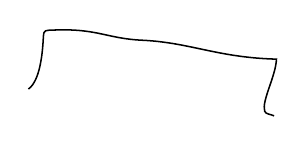
\begin{tikzpicture}[baseline=0pt]
 \draw[line width=0.55pt] (0,0.03)
 .. controls (0.15,0.14) and (0.18,0.49) .. (0.19,0.70)
 .. controls (0.19,0.78) and (0.22,0.78) .. (0.34,0.78)
 .. controls (0.88,0.80) and (1.00,0.67) .. (1.45,0.65)
 .. controls (2.06,0.62) and (2.40,0.43) .. (3.15,0.41)
 .. controls (3.14,0.19) and (2.96,-0.12) .. (3.00,-0.25)
 .. controls (3.01,-0.29) and (3.08,-0.29) .. (3.12,-0.31);
\end{tikzpicture}}
\makebox[3.15cm]{\raisebox{0.14cm}{\((24)\)}\hspace{0.22cm}\(\Sigma_*,\)}
\]
muni d'une relation d'ordre
\[
 \Sigma_{**}\subset\Sigma_*\times\Sigma_*
\]
ayant un graphe fermé\unsure{;|,} et tel que
\[
 \Sigma_{**}\xrightarrow{\operatorname{pr}_2=\mathrm{but}}\Sigma_*
\]
soit une \deleted{\unsure{plongement}}\inserted{immersion} --- plus

\margin{\textcircled{10}}
\margin{42}

\scanpage{44}
précisément, on a de plus une application croiss. et continue
\[
(2^\circ)\quad (\unsure{1|2}5)\qquad \Sigma_*\longrightarrow I
\]
(d'où
\[
\Sigma_*=\coprod_{i\in I}\Sigma_i\ ,\quad
\Sigma_{**}=\underset{i\leq j}{\deleted{\sum}\inserted{\unsure{\coprod}}}\Sigma_{ij})
\]
\deleted{\unsure{avec} $\Sigma_{ii}\simeq\Sigma_i$)}

\margin{\begin{tabular}{@{}l@{\;}l@{}}Condition \textcircled{a}&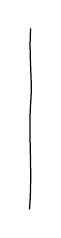
\begin{tikzpicture}[x=1cm,y=1cm,baseline=(current bounding box.center)]\draw[line width=.45pt] (0,0) .. controls (-.025,-.35) and (.025,-.65) .. (0,-.95) .. controls (-.03,-1.35) and (.025,-1.8) .. (-.015,-2.3);\end{tikzpicture}\end{tabular}}
Et on \deleted{\unsure{demande}} suppose que $\forall i,j$, \begin{tabular}[b]{@{}l@{}}\inserted{$i\leq j$}\\[-.8ex]\begin{tikzpicture}[x=1cm,y=1cm]\draw[line width=.4pt] (.6,.25) .. controls (.3,.15) and (.1,.1) .. (0,0);\end{tikzpicture}\end{tabular} le morphisme but
\[
\Sigma_{ij}\unsure{-|\longrightarrow}\Sigma_j
\]
est un \deleted{\unsure{immersion|immersement}} plongement fermé \begin{tabular}[b]{@{}l@{}}\inserted{``cylindrique''}\\[-.5ex]\begin{tikzpicture}[x=1cm,y=1cm]\draw[line width=.4pt] (0,0) .. controls (-.05,.2) and (.1,.34) .. (.4,.34) -- (1.6,.34) .. controls (1.82,.34) and (1.9,.43) .. (1.85,.57);\end{tikzpicture}\end{tabular} -- ce qui implique (par injectivité) que (25$^*$) a la propriété que si $z\in\Sigma_*$ est au dessus de $j$ et si $i\leq j$, alors il existe \uline{au plus} un $y\in\Sigma_*$ \unsure{\deleted{au}|au} \unsure{dessus|dessous} de $i$, avec $y\leq z$.
\margin{\unsure{i.e.|via} $\Sigma_*^{\leq z}\longrightarrow I^{\leq j}$ \unsure{injectif}}

Cela implique aussi
\[
(26)\qquad\Sigma_{ii}=\Sigma_i
\]
\margin{\begin{tabular}{@{}l@{\;}l@{}}\deleted{condition \unsure{b)}}&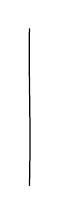
\begin{tikzpicture}[x=1cm,y=1cm,baseline=(current bounding box.center)]\draw[line width=.45pt] (0,0) .. controls (-.015,-.5) and (.02,-1.1) .. (0,-2);\end{tikzpicture}\end{tabular}}
\unsure{Car|On} \deleted{\unsure{suppose} de plus que pour $z\in$} \deleted{$\unsure{i}\unsure{\leq|<}j\unsure{\leq|<}k$,}
\[
(27)\qquad \Sigma(n)=\text{ens des drapeaux stricts de longueur }n\text{ de }\Sigma
\]
\deleted{$\Sigma_i$}
\unsure{ou|et}
\[
(27)\qquad
\begin{aligned}
\Sigma(n)&\longrightarrow\deleted{\unsure{I|\Sigma}}\operatorname{Drap}_n(I)\quad\text{(drapeaux stric}\unsure{\text{t|ts}}\unsure{)}\\
\Vert\quad&\\[-1ex]
\coprod_{\substack{(i_0<<i_n)\text{ drapeau strict en}\\ I\text{ de longueur }n}}\Sigma_{i_0- i_n}&
\end{aligned}
\]
\margin{OK}
\margin{\unsure{permet ainsi l'énoncé} de la condition (\unsure{b})}
\margin{43}

\scanpage{45}
\mspage{18}
On suppose, pour $i<j<k$
\[
(28)\qquad\Sigma_{ijk}=\Sigma_{ik}\cap\Sigma_{jk}\qquad
(\text{a priori }\Sigma_{ijk}\subset\Sigma_{ik}\cap\Sigma_{jk})
\]
\margin{Condition \textcircled{b}}
ce qui signifie aussi que $\forall z\in\Sigma_*$ au dessus d'un $k\in I$ (i.e. $z\in\Sigma_k$), l'hom. d'ens.
\[
\Sigma_*\longrightarrow I
\]
(\inserted{qui par \textcircled{a}} induit une application
\[
\Sigma_{*\leq z}\hookrightarrow I_{\leq k}
\]
\margin{\uline{injection}}
) induit
\[
(29)\qquad (\Sigma_*)_{\leq z}\hookrightarrow I_{\leq k}
\]
\margin{l'ordre de $(\Sigma_*)_z$ est \uline{induit} par celui de $I_{\leq k}$}
\margin{Ceci implique que $d,d'$ sont des drap. tels que $d''=d\cup d'$ soit un drapeau et que $d,d'$ y soient \unsure{cofinaux} i.e. $d,d'$ aient $=$ élément final $i$, alors $\Sigma_{d''}=\Sigma_d\cap\Sigma_{d'}$ dans $\Sigma_i$}

On suppose de plus que si $i,j\leq k$ n'ont pas de minorant \inserted{dans $I$}, alors
\[
\Sigma_{ik}\cap\Sigma_{jk}=\phi
\]
(si $i,j$ ont un minorant $l$, alors
\[
\Sigma_{ik}\cap\Sigma_{jk}\subset\ )
\]
\margin{Condition \textcircled{c} Gros}
\margin{Implique que si $d,d'$ sont deux drapeaux ayant $=$ élément final $k$, et si $d\cup d'$ n'est pas un drapeau, alors $\Sigma_d\cap\Sigma_{d'}=\phi$}
\margin{\textcircled{b} et \textcircled{c} impliquent que si $(d_\alpha)_\alpha$ est une famille \inserted{\unsure{finie}} de drapeaux de $I$, \deleted{\unsure{$\forall\alpha$}} \unsure{$\forall\alpha\in A$} \unsure{aient|sont} final $k$, donc les $\Sigma_{d_\alpha}\subset\Sigma_k$, alors $\bigcap\Sigma_{d_\alpha}$ est \uline{vide} si $\bigcup d_\alpha$ n'est pas un drapeau, et $=\Sigma_{\cup d_\alpha}$ sinon}

On suppose enfin que le système des $\Sigma_{ik}$ (pour $k$ fixé, \inserted{$i\in I_{<k}$}), qui sont des sous-espaces \deleted{bord} bord-ts de $\Sigma_k$, sont \uline{transversaux}, ce qui signifie (grâce : (30)\inserted{et 28,}) que si \unsure{on a} un drapeau $d=(i_{\unsure{0|1}},--i_n,k)$, alors les $\Sigma_{i_{\unsure{0|1}}k},\Sigma_{i_{\unsure{1|2}}k}\mathinner{\cdotp-}\Sigma_{i_n,k}$ dans $\Sigma_k$ sont des sous-ens \unsure{bordants|bord-ts} qui se coupent \uline{transversalement} le long de $\Sigma_d=\Sigma_{i_{\unsure{0|1}}-i_n,k}$.
\margin{Condition \textcircled{d}}
\margin{implique le $=$ dans les $\Sigma_d$\unsure{;|,} \unsure{on prend} les $\Sigma_{d'}\subset\Sigma_d$ (i.e. but pour $d'\supsetneq d$, et $d$ cofinal dans $d'$) \unsure{ce qui} \unsure{les} bord-ts\inserted{$d'=d\cup\{i\}$} \unsure{qui sont} toutes pour dans $\Sigma_d$ \unsure{liss.|lisses}}
\margin{44}

\scanpage{46}
Enfin, dans le cas équisingulier on suppose que les
\[
\Sigma_{ij}-\Sigma_i
\]
sont des \uline{fibrations} (i.e. $\Sigma_{**}\xrightarrow{s}\Sigma_*$ est une fibration), et dans le cas des strates non singulières\unsure{,|.} on suppose que les $\Sigma_i$ sont des variétés à bord (i.e. $\Sigma_*$ variété à bord) -- ce qui implique que les $\Sigma_{ji}$ \deleted{($j<i$)} tq-précédemment) sont des sous-variétés à bord du \deleted{$\Sigma_i$} bord $\dot\Sigma_i$ de $\Sigma_i$, et les $\Sigma_{ji}$ ($j<i$) forment \inserted{\unsure{les} \unsure{objt} \unsure{de|e} codim $1$ d'} une stratification cylindrique \margin{$*$}du \deleted{$\unsure{\Sigma_*}$} bord par des variétés à bord -- Alors les $\Sigma_d=\Sigma_{i_1-\, -i_n}$ sont alors des variétés à bord \deleted{\unsure{p}}. et les $\Sigma_{d'}$ ($d'\supsetneq d$, $d$ cofinal dans $d'$) \deleted{\unsure{en forment}} forment une stratification cylindrique du bord \deleted{de} $\dot\Sigma_d$ de $\Sigma_d$.
\margin{condition (e) ``équisingularité''}
\margin{[Cela implique que $\Sigma_d\longrightarrow\Sigma_{d'}$ est une fibration, si $d'\subset d$ est un \uline{segment initial} de $d$.]}
\margin{Condition (f) ``non singularité\unsure{''}}
\margin{$*$ cet ens d'indices des $d'$ s'identifie au sous-ens de
$\begin{array}{rl}
 & \inserted{\widehat{\operatorname{Drap}}(I_{\cdot<i_1})\times}\\
\widehat{\operatorname{Drap}}(I_{i_1<\cdot<i_2})\times\widehat{\operatorname{Drap}}(I_{i_2<\cdot<i_3}) & \times-\, -\times\widehat{\operatorname{Drap}}(I_{\unsure{i_{n-1}<\cdot<}i_n})
\end{array}$
où $\widehat{\operatorname{Drap}}$ désigne les drapeaux, \unsure{y.c. vides}, privé du \deleted{\unsure{drapeau}} pt unique \unsure{correspondant aux} drapeaux vides (pour $d'=d=(i_1,-i_n)$}
\margin{il s'identifie aussi à $\begin{aligned}
\operatorname{Drap}(I_{<i_1}\coprod I_{i_1<\cdot<i_2}\coprod -\,\cdot\,-\\
\qquad\cdot\,-\coprod I_{i_{n-1}<\cdot<i_n})
\end{aligned}$}

Dans le cas équisingulier-non singulier, on suppose, en plus de e) et f), que les fibres des \inserted{fibrations} $\Sigma_{ij}\longrightarrow\Sigma_i$ sont des variétés à bord -- le \deleted{\unsure{réunion}} \inserted{fibré sur $\Sigma_i$} des bords des fibres est \deleted{formé des}\inserted{\deleted{\unsure{réunion}}} stratifié par les $\Sigma_d$, où $d$ \deleted{\unsure{donne}} parcourt les drapeaux qui contiennent \uline{strictement} \deleted{$\unsure{\Sigma}$} $(i,j)$ et ont $i$ comme premier
\deleted{\unsure{élément par l'ancien produit}}
\[
\underbrace{\deleted{\widehat{\operatorname{Drap}}}}_{\substack{\text{\unsure{\deleted{drapeaux}|drapeaux}}\\\text{\unsure{\deleted{côt. vide}|côt. vide}}}}\deleted{(I_{i<\cdot<j})\times}
\underbrace{\deleted{\widehat{\operatorname{Drap}}(I_{>j})}}_{\substack{\text{\unsure{\deleted{drapeaux}|drapeaux}}\\\text{\unsure{\deleted{stricts}|stricts}}}}\unsure{,|)}
\]
\margin{Condition g)}
\margin{45}

\scanpage{47}
\mspage{19}

\deleted{\uline{privé} de $(\phi,\phi)$ (qui corresp. au drapeau $i,j$ lui $=$ \textendash{} si on ne l'excluait pas, on aurait une stratification de $\Sigma_{(i,j)}$ lui-$=$, non de son bord. Pour que $\Sigma_{ij}-\Sigma_i$ soit}
\margin{\deleted{\uline{(hyp. C.\unsure{$^{t}$|I})}}}
\deleted{lisse, il f. et s. donc que $j$ soit un successeur de $i$, et que $j$ soit \unsure{maximal} dans $I$}

élément (pour être fibré sur $\Sigma_i$) et $j$ comme dernier (pour être \unsure{contenus|contenu} ds $\Sigma_{ij}$) s'\unsure{ident} donc \inserted{$\simeq$} $\operatorname{Drap}(I_{i< <j})$. Il est vide ssi $j$ est un successeur de $i$, qui est donc la condition pour que $\Sigma_{ij}\unsure{-|\longrightarrow}\Sigma_i$ soit lisse.

Plus généralement, si $d\subsetneq d'$ est un segment initial, la fibration $\Sigma_{d'}\longrightarrow\Sigma_d$ est à fibres des variétés à bord, et le fibré des bords est stratifié cylindriquement par les $\Sigma_{d''}$ où $d''\supsetneq d'$ (pour que $\Sigma_{d''}\overset{\deleted{\unsure{\alpha}}}{\hookrightarrow}\Sigma_{d'}$) est tel que $d'$ soit cofinal dans $d''$ (pour que $\Sigma_{d''}\hookrightarrow\Sigma_{d'}$) et que $d$ soit segment initial dans $d''$ (pour que $\Sigma_{d''}\longrightarrow\Sigma_{d'}$ soit fibrant) i.e. \deleted{\unsure{si $d$ est le|si on est le}} \inserted{si $d'=(i_1-i_n)$}
$d=(i_1,-i_p)$, \deleted{\unsure{alors|donc} $d''$ \unsure{est de la forme}} d'où $d'=d\coprod d'_0$
\deleted{plus \unsure{grand élément} de $d_p$ et plus \unsure{grand élément}}
avec $d'_0=(i_{p+1},i_{p+2}\mathinner{\cdot-}i_n)$, alors les $d''$ correspondent aux

\noindent\begin{minipage}{\linewidth}
\leavevmode\rlap{\begin{tikzpicture}[overlay,x=1cm,y=1cm]
  \draw[line width=.35pt] (-.12,.16) -- (-.12,-1.03) .. controls (-.10,-1.17) and (.06,-1.20) .. (.27,-1.20) -- (8.15,-1.17) .. controls (8.52,-.98) and (8.19,-.68) .. (8.20,-.52);
  \draw[line width=.35pt] (2.05,-1.15) .. controls (3.51,-.61) and (5.85,.35) .. (5.69,-.16) .. controls (5.65,-.36) and (4.75,-.92) .. (5.03,-.83) .. controls (6.26,-.41) and (6.62,-.27) .. (7.16,-.38);
\end{tikzpicture}}
\deleted{\unsure{par $d'$} (\unsure{donc} $\alpha\leq\beta$), \unsure{ce sont} les drapeaux \unsure{ayant|où}}\\
\deleted{$\beta$ comme plus grand élément, et \unsure{formé d'indices}}\\
\deleted{\unsure{forme} $d\coprod d''_0$, où $d''_0\subset I_{\cdot>\alpha}$}
\end{minipage}

\inserted{\unsure{les|des} drapeaux \deleted{\unsure{finis}} $d''_0\subset I_{\cdot>i_p}$\unsure{)|,}} contenant \deleted{\unsure{$d_0$|les}} strictement $d'_0$ et tels que $d'_0$ soit cofinal dans $d''_0$, \deleted{\unsure{c'est donc un}} \inserted{l'un de ces $d''_0$, ou l'ens des $d''_0$, est en} corresp. biunivoque avec
\[
\operatorname{Drap}\bigl(I_{i_p<\cdot<i_{p+1}}\deleted{\unsure{\}|)}}\coprod I_{i_{p+1}<\cdot<i_{p+2}}\coprod\mathinner{-\,-\,\cdot}\coprod I_{i_{n-1}<\cdot<i_n}\bigr)
\]
\margin{46}

\scanpage{48}
On a lissité (à tous les coups) ssi \deleted{\unsure{$i_p$|pour}} la suite $i_p\ i_{p+1}-\, -\,i_n$ (à partir de $i_p$, pas de $i_1$ !) est stricte, i.e. chaque terme \inserted{(sauf le premier)} est successeur \inserted{dans $I$} du précédent.

11. \uline{Digression : où on laisse tomber} $I$.

Soit donné un ens. ordonné topologique, i.e. un \deleted{espace topologique} ens. ordonné $\Sigma=\Sigma(0),\Sigma(1)$, où $\Sigma(0)$ est un espace topologique, $\Sigma(1)$ une partie fermée de $\Sigma(0)\times\Sigma(0)$, qui soit le graphe d'une relation d'ordre. On suppose
\margin{On retient \unsure{ce} cas}

\textcircled{a}\quad $\Sigma(1)\xrightarrow{\mathrm{but}}\Sigma(0)$ est une immersion localement bordante, et propre (donc fini)

\deleted{\textcircled{b}} Cela implique que $\Sigma(0)\xrightarrow{\mathrm{diag}}\Sigma(1)$ est un isomorphisme sur une partie ouverte et fermée. Soit $\Sigma^{<}(1)$ le complémentaire de l'image, i.e l'ens où \unsure{une|on a} des inégalités strictes $i<j$. On désigne par $\Sigma^{<}(n)$ l'espace des drapeaux \uline{stricts} $i_0<i_1-\, -\,<i_n$ de longueur $n$. Les. $\Sigma^*(n)$ \deleted{\unsure{sont}} \inserted{\unsure{forment}} un espace \inserted{pré}\deleted{semi}-simplicial (\uline{NB} pas d'applications de dégénérescence, \deleted{\unsure{car par}} ils sont dans les $\Sigma(n)\mathinner{\cdotp\cdotp-}$). \unsure{\deleted{Les}|Les} Si on a un
\margin{47}
